\documentclass[11pt]{article}
\usepackage{amsmath}
\usepackage{amssymb}
\usepackage{graphicx}
\usepackage{fancyhdr}
\usepackage{enumerate}
\usepackage{listings}
\usepackage{titlesec}
\usepackage{mathtools}
\usepackage[colorlinks=true,urlcolor=blue]{hyperref}

\usepackage{color}

\definecolor{dkgreen}{rgb}{0,0.6,0}
\definecolor{gray}{rgb}{0.5,0.5,0.5}
\definecolor{mauve}{rgb}{0.58,0,0.82}

\lstset{frame=tb,
  language=Java,
  aboveskip=3mm,
  belowskip=3mm,
  showstringspaces=false,
  columns=flexible,
  basicstyle={\small\ttfamily},
  numbers=none,
  numberstyle=\tiny\color{gray},
  keywordstyle=\color{blue},
  commentstyle=\color{dkgreen},
  stringstyle=\color{mauve},
  breaklines=true,
  breakatwhitespace=true,
  tabsize=3
}



\titlespacing{\subsubsection}{0pt}{0pt}{0pt}

% No page numbers
%\pagenumbering{gobble}

% MARGINS (DO NOT EDIT) ---------------------------------------------
\oddsidemargin  0.25in \evensidemargin 0.25in \topmargin -0.5in
\headheight 0.2in \headsep 0.1in
\textwidth  6.5in \textheight 9in
\parskip 1.25ex  \parindent 0ex \footskip 20pt
% ---------------------------------------------------------------------------------

% HEADER (DO NOT EDIT) -----------------------------------------------
\newcommand{\problemnumber}{0}
\newcommand{\myname}{name}
\newfont{\myfont}{cmssbx10 scaled 1000}
\pagestyle{fancy}
\fancyhead{}
\fancyhead[L]{\myfont Question \problemnumber, Homework 1, CME241}
%\fancyhead[R]{\bssnine \myname}
\newcommand{\newquestion}[1]{
\clearpage % page break and flush floats
\renewcommand{\problemnumber}{#1} % set problem number for header
\phantom{}  % Put something on the page so it shows
}
% ---------------------------------------------------------------------------------


\newcommand{\spike}[2]% #1 = size of spike, #2 = centered text
{\bgroup
  \sbox0{#2}%
  \rlap{\usebox0}%
  \hspace{0.5\wd0}%
  \makebox[0pt][c]{\rule[\dimexpr \ht0+1pt]{0.5pt}{#1}}% top spike
  \makebox[0pt][c]{\rule[\dimexpr -\dp0-#1-1pt]{0.5pt}{#1}}% bottom spike
  \hspace{0.5\wd0}%
\egroup}


% BEGIN HOMEWORK HERE
\begin{document}

% Question 1(a)
\newquestion{1(a)}

State Space $S = \{0, 1, 2, 3, \ldots, 100\}$

In other words, the state space is the set of integers from 0 to 100, inclusive.

% Question 1(b)
\newquestion{1(b)}

This is a lot to write out, so I will just explain the logic of my code.

I start by initializing a 101 by 101 matrix of zeros. The final row/column represents the terminal state of winning the game. We start by saying that starting at i=0 and given a state i, states i+1, i+2,...,i+6 receive 1/6 probability corresponding to the sides of a fair die. However, we also don't give probability for state i>100, since that would be out-of-bounds. We adjust the terminal state transition probability upwards for states 95 through 99 since multiple die roll outcomes become associated with winning. Finally, we account for the snakes and ladders by giving all the columnar probability from the start of the snake/ladder to the end of the snake/ladder and then zeroing out the starting square probability. This represents how you can't really have a state equal to the starting square of a snake/ladder since you will immediately teleport to ending square.

\begin{lstlisting}
# Create transition matrix
# Start with uniform dist of moving 1 to 6 spaces forward
transition_matrix = np.zeros((101,101))
for i in range(100):
    for j in range(i+1, min(i+7, 101)):
        transition_matrix[i, j] = 1/6
# Prob of winning (term state) is 1 minus sum of probs on non-term states
transition_matrix[:,-1] = 1 - np.sum(transition_matrix[:, :-1], axis=1)
# Create mapping for the ladders and snakes
ls_dict = {1:38, 4:14, 8:10, 21:42, 
    28:76, 50:67, 71:92, 80:99,
    97:78, 95:56, 88:24, 62:18, 48:26, 
    36:6, 32:10}
# Edit transition matrix according to the mapping
for start_sq, end_sq in ls_dict.items():
    transition_matrix[:, end_sq] += transition_matrix[:, start_sq]
    transition_matrix[:, start_sq] = 0
\end{lstlisting}

% Question 1(c)
\newquestion{1(c)}
Done in code.

% Question 1(c)
\newquestion{1(d)}
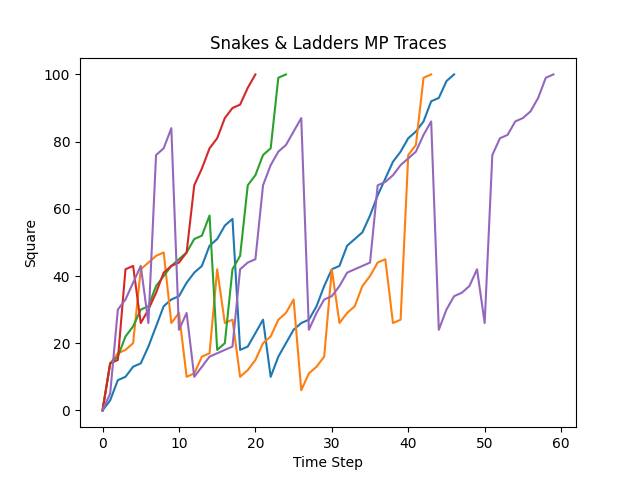
\includegraphics[scale=0.8]{sample_traces.png}

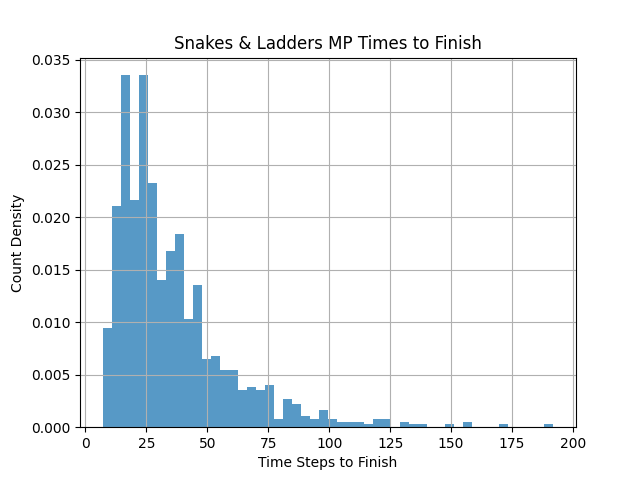
\includegraphics[scale=0.8]{times_to_finish.png}
% Question 1(e)
\newquestion{1(e)}
The expected number of rolls to finish the game from the beginning is 34.0339. To calculate this number, we set up a reward function which just deterministically returns 1 for every non-terminal state. We also set gamma to 1.0. This allows us to count the time-steps.

\newpage

% Question 2(a)
\newquestion{2(a)}

I think of the lilypads as representing integers, so:

State Space $S = \{0, 1, 2, 3, \ldots, 10\}$

In other words, the state space is the set of integers from 0 to 10, inclusive.

The transition probabilities are that given that you are at state s, you have uniform transition probability over states s' where s'>s. We can create a transition matrix for the non-terminal states as described by my code:

\begin{lstlisting}
transition_matrix = np.zeros((10, 10))
for i in range(10):
    transition_matrix[i, i+1:] = 1/(10-i)
\end{lstlisting}

% Question 2(b)
\newquestion{2(b)}
Define the transition matrix $P \in R^{n+1xn+1}$ using the code from part (a). The reward vector $\vec{r}$ is just a vector of ones and is of dimension n+1. We also have the $\vec{e}_1 = [1, 0, \ldots,0]^T$ of dimension n+1. Then we have:

$$\text{E(hops from start)} = \vec{e}_1^T(I-P)^{-1}\vec{r}$$

So then:
Expected number of hops to reach other side: 2.928968253968254

Also shown in code.

% Question 2(c)
\newquestion{2(c)}
Let $n$ be the number of lilypads and $y_n$ be the number of hops needed to get across given $n$ lilypads.
The closed form solution is:
$$\text{E}(y_n) = \sum_{j=0}^n \frac{1}{j+1}$$

We can prove by induction. When n=0 it is trivial that $\text{E}(y_0) = 1 / (0+1) = 1$. It is also easy to show that the closed form solution works for n=1 (proving the base case) by using the following recursion:
$$\text{E}(y_n) = 1  + \frac{1}{n+1} \sum_{i=0}^{n-1}\text{E}(y_i)$$
To prove the inductive step, we assume that the closed form solution holds for all $i<n$, so then:
$$\text{E}(y_n) = 1  + \frac{1}{n+1} \sum_{i=0}^{n-1} \sum_{j=0}^i \frac{1}{j+1}$$
Reorder the sum:
$$\text{E}(y_n) = 1  + \frac{1}{n+1} \sum_{j=0}^{n-1} \sum_{i=j}^{n-1} \frac{1}{j+1}$$
$$\text{E}(y_n) = 1  + \frac{1}{n+1} \sum_{j=0}^{n-1} \frac{n-1-j+1}{j+1}$$
$$\text{E}(y_n) = 1  + \frac{1}{n+1} \sum_{j=0}^{n-1} \frac{n+1}{j+1} - 1$$
$$\text{E}(y_n) = 1  + \frac{1}{n+1} ((\sum_{j=0}^{n-1} \frac{n+1}{j+1}) - n)$$
$$\text{E}(y_n) = 1  - \frac{n}{n+1}  + \sum_{j=0}^{n-1} \frac{1}{j+1}$$
$$\text{E}(y_n) = \frac{1}{n+1} + \sum_{j=0}^{n-1} \frac{1}{j+1}$$
$$\text{E}(y_n) = \sum_{j=0}^{n} \frac{1}{j+1}$$

Thus we prove the closed form solution by induction.

\end{document}
